\documentclass[article,10pt]{article}
% ,two column
%\usepackage[utf8]{inputenc}
%\usepackage[ruled,vlined]{algorithm2e}
\usepackage{graphicx}  % Required for including images
\usepackage{caption}   % For customizing captions
\usepackage{subcaption} % For subfigures
\usepackage{subfig}
\usepackage{float} % Add this line for the H option
\usepackage{multicol}
\usepackage[margin=2cm]{geometry} 
\usepackage{titlesec}
\usepackage{algorithm}
\usepackage[noend]{algpseudocode}
\usepackage{array}
\usepackage{setspace}
\usepackage{booktabs}
%\usepackage[authoryear]{natbib}
\usepackage{url}

\setlength{\parindent}{0pt}

\date{ }
% \title{Comparison Between Selection Sort And TimSort}
\title{Comparative Analysis of Selection Sort and TimSort}

\author
{
  \begin{tabular}[t]{c@{\extracolsep{12mm}}c@{\extracolsep{12mm}}c}
    {\it Shahriar Rizvi} & {\it Tanvir Mahamood} & {\it Rushnan Reaz}\\
    \small Department of CSE & \small Department of CSE & \small Department of CSE\\
    \small RUET & \small RUET & \small RUET\\
    \small 2003104@student.ruet.ac.bd & \small 2003062@student.ruet.ac.bd & \small 2003101@student.ruet.ac.bd\\
    \\
    {\it Jaeed Mahmud} & {\it Nafees Ahamed} & {\it Rakebul Hasan Nur}\\
    \small Department of CSE & \small Department of CSE & \small Department of CSE\\
    \small RUET & \small RUET & \small RUET\\
    \small 2003074@student.ruet.ac.bd & \small 2003079@student.ruet.ac.bd & \small 2003066@student.ruet.ac.bd\\
  \end{tabular}
}

% \begin{tabular}[t]{c@{\extracolsep{20mm}}c@{\extracolsep{20mm}}c}
% {\it Author-1} & {\it Author-2} & {\it Author-3}\\
% Affiliation-1 & Affiliation-2 & Affiliation-3\\
% Address-1 & Address-2 & Address-3\\
% e-mail-1 & e-mail-2 & e-mail-3\\
% \end{tabular}

% \begin{tabular}[t]{c@{\extracolsep{20mm}}c@{\extracolsep{20mm}}c}
% {\it Author-4} & {\it Author-5} & {\it Author-6}\\
% Affiliation-4 & Affiliation-5 & Affiliation-6\\
% Address-4 & Address-5 & Address-6\\
% e-mail-4 & e-mail-5 & e-mail-6\\
% \end{tabular}


\titleformat{\section}[block]{\normalfont\Large\bfseries}{\Roman{section}.}{1em}{}


\begin{document}
\maketitle
%


\begin{abstract}
\noindent
This article presents two popular sorting algorithms naming Selection Sort and TimSort. Selection Sort is comparable to a brute force approach, while TimSort employs a divide-and-conquer strategy by incorporating merge sort. In particular, both merging sort and Selection Sort share the same best-case and worst-case complexities $O(nlogn)$ and $O(n^2)$, respectively. The goal of this article is to discuss about the sorting techniques, comparing their performance with real life data, discussing about complexity analysis in terms of best case and worst case and space or auxiliary complexity. These discussions will be enough to make a comparison between these algorithms.


\end{abstract}
%
\begin{multicols}{2}
\section{Introduction}
% In algorithmic design and optimization, sorting algorithms play a pivotal role in influencing the efficiency and performance of a myriad of computational processes. This article embarks on a detailed comparative analysis between Selection Sort\cite{Knuth-Selection}  and TimSort\cite{peters2015TimSort}, two sorting algorithms that have found widespread use in diverse computing environments.

% Selection Sort, a straightforward and intuitive algorithm, is frequently featured in introductory computer science courses as a foundational concept and has become a staple in various sorting implementations. However, its simplicity comes with trade-offs, particularly in terms of time complexity. On the other hand, TimSort, a hybrid sorting algorithm derived from Merge Sort and Insertion Sort, incorporates sophisticated techniques to enhance performance across various data distributions.

Sorting algorithms are essential to algorithmic design and optimization because they have a significant impact on the effectiveness and performance of numerous computer operations. In this article, TimSort\cite{peters2015TimSort} and Selection Sort\cite{Knuth-Selection}—two sorting algorithms that have been widely used in a variety of computing environments—are thoroughly compared.\\

An easy-to-understand algorithm, selection sort is a mainstay in many sorting implementations and is commonly taught as a core topic in introductory computer science classes. But there are trade-offs associated with its simplicity, especially when it comes to time complexity. Conversely, TimSort is a hybrid sorting algorithm that combines advanced strategies to improve performance on a range of data distributions. It is derived on Merge Sort and Insertion Sort.\\

% The primary objective of our investigation is to elucidate the running time characteristics of Selection Sort and TimSort under different scenarios, ranging from best- to worst-case conditions. Additionally, we delve into the space-time trade-offs inherent in these algorithms, shedding light on their memory requirements and overall efficiency.

% correction>>To ensure a robust and meaningful analysis, we draw upon datasets obtained from reputable sources specializing in machine learning datasets. Furthermore, locally generated data are incorporated to simulate real-world scenarios, providing a comprehensive understanding of how these sorting algorithms perform in practical applications.

Our investigations' main intention is to clarify Selection Sort and TimSorts' running time characteristics in a variety of scenarios, from the best to the worst. We also explore the space-time trade-offs that these algorithms entail, providing insight into their overall efficiency and memory needs.\\

We use datasets from reliable sources that specialize in machine learning datasets to provide a solid and insightful analysis. Moreover, locally generated data are integrated to emulate real-world situations, offering a thorough comprehension of the performance of various sorting algorithms in real-world scenarios.\\

% As we navigate through the intricacies of algorithmic complexity, we aim to equip researchers, developers, and educators with valuable insights into the comparative strengths and weaknesses of Selection Sort and TimSort. By offering a nuanced perspective on its performance characteristics, this article contributes to the ongoing discourse on algorithmic efficiency and aids in informed decision-making when selecting sorting algorithms for specific computational tasks.<<correction

We hope to provide researchers, developers, and educators with useful insights about the relative advantages and disadvantages of TimSort and Selection Sort as we traverse the complexities of algorithmic complexity. This article adds to the current discussion on algorithmic efficiency by providing a nuanced viewpoint on its performance characteristics. It also facilitates the process of making well-informed decisions when choosing sorting algorithms for particular computational jobs.


\section{Background Study}


\begin{center} \underline{\textbf{Selection Sort}} \end{center}
\begin{figure*}[t!]\centering \setstretch{0.9}
    \begin{tabular}{p{3cm} p{1cm} p{4cm}}
      
        \textbf{Algorithm} & \textbf{Cost} & \textbf{Number of Operations} \\
        
        \begin{verbatim}
selectionSort(arr: A)
    for i from 1 to A.length-1 do
        minIndex = i
        for j from i+1 to A.length do
            if A[j] < A[minIndex] then
                minIndex = j
            end if
        end for
        if A[i] < A[minIndex] then
		            Temp = A[i]
            A[i] = A[minIndex]
            A[minIndex] = temp
    end for
        \end{verbatim}
        &
        \begin{verbatim}

C1
c2

c3



c4
c5
c6
c7
        \end{verbatim}
        &
        \begin{verbatim}

n
(n-1)

(n-1)+(n-2)+…+3+2+1
= n(n-1)/2 


(n-1)
(n-1)
(n-1)
(n-1)

        \end{verbatim}

        \multicolumn{3}{p{10.5cm}}{Total Complexity: $c_1 n + c_2(n-1) + c_3n(n-1)/2 + c_4(n-1) + c_5(n-1) + c_6(n-1) + c_7(n-1)$}
    \end{tabular}
    %\caption{Analysis of Selection Sort Algorithm}
    %\label{tab:selectionsort}
\end{figure*}
Selection Sort\cite{Knuth-Selection} is a simple but inefficient algorithm for sorting. In this algorithm, we have to find the smallest element of the array and move it to the front of the array. We need to use a linear search technique to find the smallest element. Here, moving an element means swapping. After that, we find the second smallest element and move it to its actual position. This process should continue until all the elements are in their right places. At that time, the array will be completely sorted in ascending order.Suppose ‘A’ is given as an array that is to be sorted. The array is one indexed.\\
%\end{multicols}





%\begin{multicols}[2]
    

\textbf{Worst Case Time Complexity}: This can be achieved when we need to sort elements in ascending order, but the array is initially in descending order. The outer and inner loops do not depend on the order of arrangement of the array. It is the common cost for both the best and worst case. The only difference is the ‘SWAP’ operation. During each iteration, the swap operation will be performed.
the overall time cost:

$T(n) = c_1n + c_2(n-1) + c_3n(n-1) / 2 + c_4(n-1) + c_5(n-1) + c_6(n-1) + c_7(n-1)
= (c_3/2)n^2 + (c_1+c_2-c_3/2+c_4+c_5+c_6+c_7)n + (-c_2-c_4-c_5-c_6-c_7)$\\

This running time can be expressed as\\ $T(n) = an^2 + bn + c$

Here, $a = c_3/2, b = c_1+c_2-c_3/2+c_4+c_5+c_6+c_7$ and $c = -c_2-c_4-c_5-c_6-c_7$.\\
So, the worse case complexity is O($n^2$)\\


\textbf{Best Case Time Complexity}: As mentioned before, the number of iterations of the outer and inner loops are free from the order of array arrangement, we should only focus on the swap operation. The best case happens when the array is already sorted in ascending order as we wanted. At that time, no swap operation was needed during the total iterations. Because the $i^{th}$ element is smaller than all $j^{th}$ elements. Thus, the total time cost will be reduced slightly. That is:\\
$T(n) = c_1n + c_2(n-1) + c_3n(n-1) / 2 + c_4(n-1)
= (c_3/2)n^2 + (c_1+c_2-c_3/2+c_4)n + (-c_2-c_4)$\\
This running time can be expressed as \\
$T(n) = a’n^2 + b’n + c’$\\
Here, $a’ = c_3/2, b = c_1+c_2-c_3/2+c_4$ and $c = -c_2-c_4$.
So, the best case complexity: O($n^2$)\\
In short, time Complexity is O($n^2$) for both best-case and worst-case. But the constant factor during the best case is smaller than in the worst case.\\

\textbf{Auxiliary Space}: As no extra space is needed to sort the array except the variable 'Temp' for swapping, the space complexity is O(1).\\

\textbf{Stability}: The stable order preserves the original order of the input set. The Selection Sort is unstable. Here is an example.\\
Suppose that the array is [5 3 4 5 2 6 8]. \\
Let's distinguish the two 5's as 5(a) and 5(b). So, our array is: [5(a) 3 4 5(b) 2 6 8].\\
After the first iteration, 5(a) will be swapped with 2. So, our array becomes: [2 3 4 5(b) 5(a) 6 8]\\
Now, the array is sorted. We have seen that 5(a) comes before 5(b) in the initial array. But after sorting.
Since now our array is in sorted order, we see that 5(a) comes before 5(b) in the initial array but not in the sorted array. So, we can see that the Selection Sort is not stable.\\
In this paper, we will use the Selection Sort algorithm given in \cite{Knuth-Selection}. 


% \begin{figure*}[b!]\centering \setstretch{0.9} 
%     \begin{tabular}{p{7cm}p{1cm}p{4cm}}
      
%         \textbf{Algorithm} & \textbf{Cost} & \textbf{Number of Operations} \\
        
%         \begin{verbatim}
% selectionSort(arr: A)
%     for i from 1 to A.length-1 do
%         minIndex = i
%         for j from i+1 to A.length do
%             if A[j] < A[minIndex] then
%                 minIndex = j
%             end if
%         end for
%         if A[i] < A[minIndex] then
% 		            Temp = A[i]
%             A[i] = A[minIndex]
%             A[minIndex] = temp
%     end for
%         \end{verbatim}
%         &
%         \begin{verbatim}

% C1
% c2

% c3



% c4
% c5
% c6
% c7
%         \end{verbatim}
%         &
%         \begin{verbatim}

% n
% (n-1)

% (n-1)+(n-2)+…+3+2+1
% = n(n-1)/2 


% (n-1)
% (n-1)
% (n-1)
% (n-1)

%         \end{verbatim}

%         \multicolumn{3}{p{10.5cm}}{Total Complexity: $c_1 n + c_2(n-1) + c_3n(n-1)/2 + c_4(n-1) + c_5(n-1) + c_6(n-1) + c_7(n-1)$}
%     \end{tabular}
%     %\caption{Analysis of Selection Sort Algorithm}
%     %\label{tab:selectionsort}
% \end{figure*}


\begin{center} \underline{\textbf{TimSort}} \end{center}
TimSort, a hybrid algorithm was created in 2002 with an emphasis on real-world data by Tim Peters\cite{peters2015TimSort}. Python, the Java standard library, GNU Octave, and the Android operating system utilize different refined versions of TimSort as their default sorting method.\\
Before TimSort, QuickSort was widely used as the fastest algorithm for sorting elements. In the work \cite{Cook-et-al:1980}, they proposed a hybrid algorithm which is a synergy of QuickerSort\cite{quicker} and Straight Insertion Sort\cite{Knuth-StInsertion} for almost sorted elements\cite{Cook-et-al:1980}. In 2002, Tim Cook proposed a stable merge sort that was claimed to be faster than any other algorithms for sorting real-world elements, as sorting real-world elements rarely has a high out-of-order percentage \cite{peters2015TimSort}.  Auger et al.\cite{Auger-2015} were the first to prove TimSort in their work in 2015. Further improvements can be found in \cite{Auger-2019}  and \cite{gouw-java}.
The refinement proposed in the work of Stijn de Gouw\cite{gouw-java} is now used in Python. But, the Java standard library uses the first version of TimSort by adjusting tuning values which was exposed in \cite{gouw-java}. 
\\
Timsort mainly uses InsertionSort and Merge Sort. In TimSort, if the algorithm tends to find sub-problems ranging from 32 to 64 elements\cite{peters2015TimSort}. This approach stops dividing operations and the number of levels of recurrence is reduced. Now the remaining subarray is sorted using Insertion Sort. After sorting each sub-arrays, the algorithm merges these sub-arrays. The constant factor of the insertion sort is lower than the merge sort. It is known that Insertion Sort executes more efficiently than Merge Sort for a small number of elements\cite{Cook-et-al:1980}. That’s why adding this new feature can increase runtime quality. So, the number of levels is decreased from $\log(n)$ to $(\log(n)-x)$, here, x is the number of levels that are ignored because of Insertion Sort.
\\
Now, the algorithm is further modified to improve the execution time by introducing 'Run'. ‘Run’ is a sorted sublist of elements among the elements\cite{Knuth-Merge}. If we find a sub-array that is already sorted, we do not divide it further, and this sub-array will be recognized as 'run'. The ‘Run’ has to be strictly in Ascending order\cite{peters2015TimSort}. ‘Run’s do not need any sorting algorithm. All 'Run' and the other smallest subarrays are merged. Thus, the overall complexity is improved.

\textbf{Best Case Time Complexity}: In the best case scenario, the array is already sorted and the entire array will work as ‘Run’. So, we do not need to take a divide-and-conquer approach. Simply, the time complexity is O(n).\\

\textbf{Worst Case Time Complexity}: In the worst case scenario, the Time complexity is O($n\log(n)$) which is proven in the work of Auger et al.\cite{Auger-2015, Auger-2019}.\\

\textbf{Auxiliary Space}: The auxiliary (or extra) space complexity of TimSort is O(n). TimSort uses additional space for temporary storage and various data structures during the sorting process. The primary data structure is the auxiliary array used for merging the sorted runs.TimSort may use a stack to keep track of the runs and their indices during the sorting process.\\ 

\textbf{Stability}: TimSort is stable because it uses a merging mechanism that preserves the relative order of equal elements during the sorting process. It also employs Insertion Sort for small sequences, which is inherently stable. The comparison and swapping criteria in TimSort are designed to maintain stability, ensuring that equal elements retain their original order.\\\\

\begin{center} \underline{\textbf{Comparison}} \end{center}
\begin{itemize}
	\item TimSort is very optimized. Its best-case and worst-case time complexity is O(n) and O($n\log(n)$) respectively. On the other hand, Selection Sort is very inefficient and runs in O($n^2$) for both worst and best cases.
	\item Selection Sort uses no extra space for sorting. It is space-optimized. TimSort is not space-optimized.
	\item TimSort is a stable sorting algorithm. Selection Sort is unstable.
\end{itemize}







%%%%%%%%%%%%%%%%%%%%%%%% Result and Analysis %%%%%%%%%%%%%%%%%%%%%%%%%%%%

\section{Results and Analysis}

% In this section, we present the results of our time analysis comparing Selection Sort and TimSort on datasets of different sizes (900, 9000, and 100000 elements). Additionally, we include visualizations of the theoretical time complexities represented by \(O(n^2)\) and \(O(n \log n)\) graphs for reference.\\

The algorithms under consideration were implemented in the Python programming language and rigorously tested using random sequence inputs of varying lengths, including 900, 9000, and 100000 elements. The experiments were carried out in a computing environment equipped with an 11$^{th}$ generation Intel(R) Core(TM) i7-1195G7 processor operating at 2.90GHz, complemented by 16GB RAM.\\

\noindent

\begin{figure*}[t!]
	\centering
	\begin{subfigure}{0.4\textwidth}
		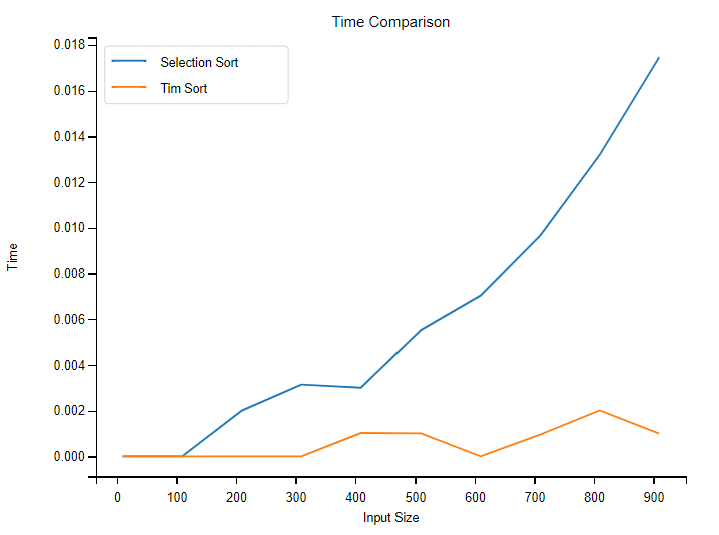
\includegraphics[scale=0.25]{Images/900_time_comp.png}
		\caption{For data size: 0 to 900}
		\label{d900}
	\end{subfigure}
 \hfill
	\begin{subfigure}{0.4\textwidth}
		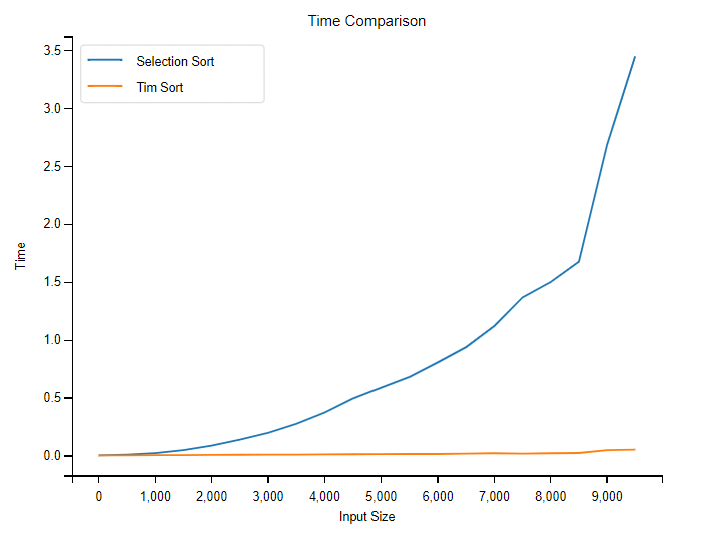
\includegraphics[scale=0.25]{Images/9k_time_comp.png}
		\caption{For data size: 0 to 9000}
		\label{d9k}
	\end{subfigure}
        \begin{subfigure}{0.4\textwidth}
		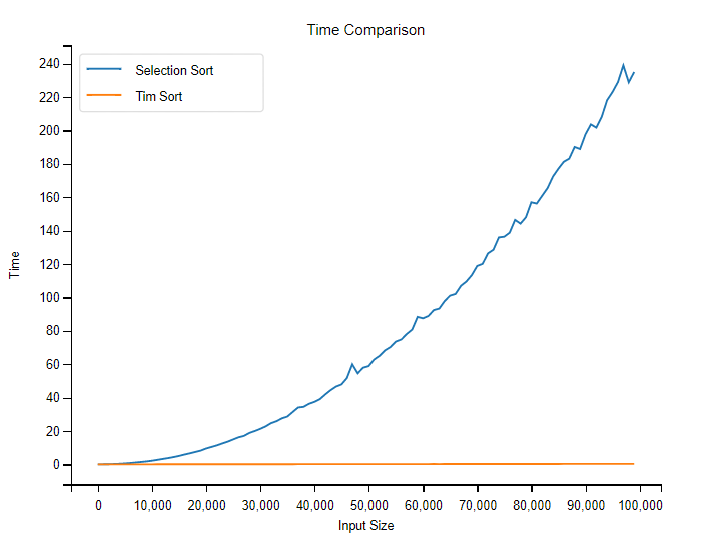
\includegraphics[scale=0.25]{Images/100k_time_comp.png}
		\caption{For data size: 0 to 100,000}
		\label{d100k}
	\end{subfigure}
\hfill
        \begin{subfigure}{0.4\textwidth}
		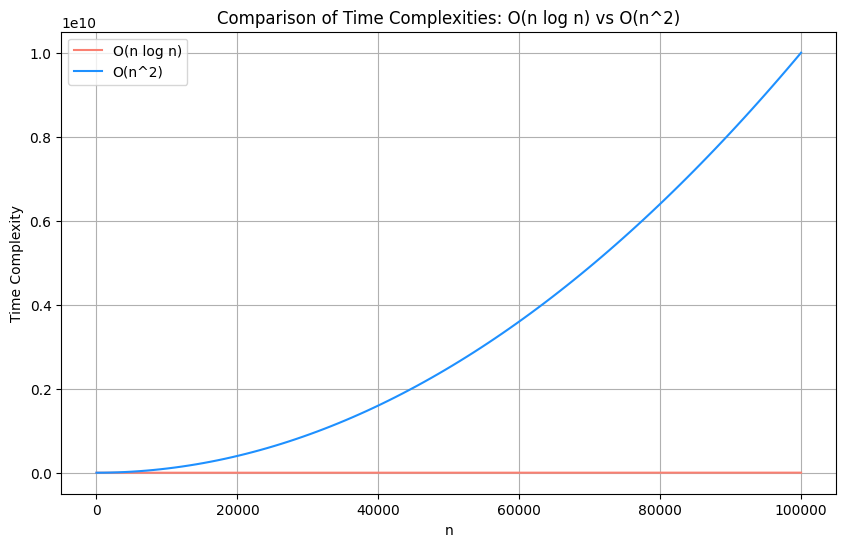
\includegraphics[scale=0.25]{Images/actual_Function.png}
		\caption{For theoretical \(O(n^2)\) and \(O(n \log n)\) }
		\label{fig:theoretical_complexities}
	\end{subfigure}
 
	\caption{Experimented and Theoretical Time Comparison between Selection and TimSort}
 
\end{figure*}

% \textbf{Time Analysis}
\begin{center} \underline{\textbf{Time Analysis}} \end{center}
We conducted a comprehensive time analysis to assess the performance of Selection Sort and TimSort across varying dataset sizes. The results are illustrated in Figures \ref{d900}, \ref{d9k}, and \ref{d100k} for data set sizes of 900, 9000, and 100000 elements, respectively. The observed trends indicate distinctive behaviors in the growth of execution time as the dataset size increases. In particular, the \textbf{Selection Sort} algorithm (pictured in blue) exhibits exponential growth, showcasing a substantial increase in execution time with larger datasets. In contrast, the \textbf{TimSort} algorithm (pictured in salmon) demonstrates a more moderate growth rate, suggesting its efficiency in handling larger data sets.

A particularly noteworthy observation is the discernible difference in the curves for higher input sizes, such as 900 to 9000 and 100,000. In this range, the visual contrast between the performance of Selection Sort and TimSort becomes more pronounced, further emphasizing the superior scalability of TimSort for substantial datasets. 

As depicted in the figures, TimSort consistently outperforms Selection Sort across all dataset sizes. The divide-and-conquer strategy employed by TimSort demonstrates its efficiency, particularly as the dataset size increases.





%\end{multicols}





%\begin{multicols}{2}
\vspace{ }
\noindent
% \textbf{Theoretical Time Complexities}
\begin{center} \underline{\textbf{Theoretical Time Complexities}} \end{center}

To provide a theoretical context for our empirical findings, we include graphs representing the time complexities of \(O(n^2)\) and \(O(n \log n)\) in Figure \ref{fig:theoretical_complexities}. Which is generated in Python using 'matplotlib' library. 

The theoretical complexities serve as a reference point, confirming that the observed performance aligns with the expected behaviors of Selection Sort and TimSort.

% \end{multicols}
% \begin{figure}[b!]
% \centering
%   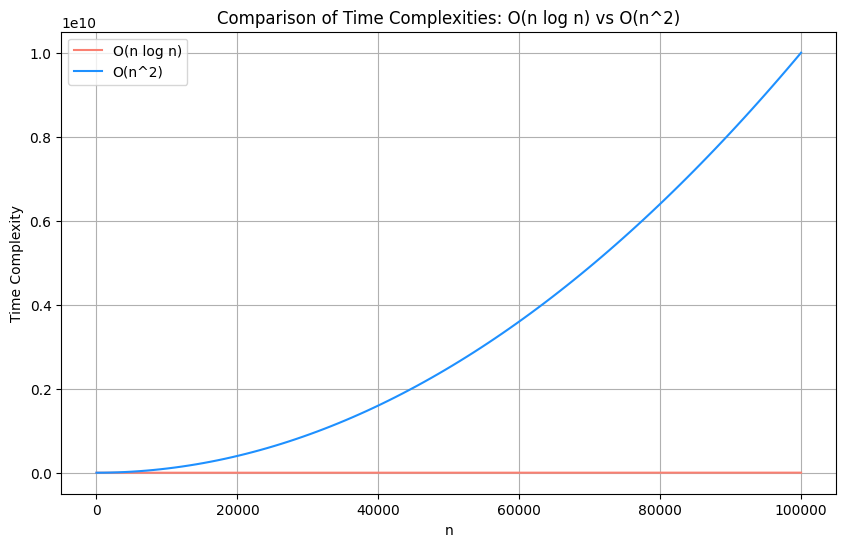
\includegraphics[width=0.4\textwidth]{Images/actual_Function.png}
%   \caption{Theoretical time complexities: \(O(n^2)\) and \(O(n \log n)\).}
  
%   \label{fig:theoretical_complexities}
% \end{figure}

% \begin{multicols}{2}



In summary, our empirical results and theoretical considerations collectively suggest that TimSort is a more efficient sorting algorithm compared to Selection Sort, especially in scenarios with larger datasets.
% \end{multicols}


% \begin{multicols}{2}

\section{Conclusion}
This paper represents two sorting algorithms (Selection Sort and TimSort), their sorting techniques, time complexity, and performance. To compare sorting algorithms, the time complexity is the main consideration. It analyzes the time complexity for the worst and the best cases. Moreover, several data sets are used to compare the performance of these two algorithms. It upholds the comparison of performance by graph, which highlights the high efficiency of TimSort for a large number of elements that are to be sorted. 


\bibliographystyle{acm}
\bibliography{mybib2}


\end{multicols}
\end{document}